\iffalse
\documentclass[book,11pt]{IEEEtran}
\usepackage{setspace}
\usepackage{gensymb}
\singlespacing
\usepackage[cmex10]{amsmath}
\usepackage{amsthm}
\usepackage{mathrsfs}
\usepackage{txfonts}
\usepackage{stfloats}
\usepackage{bm}
\usepackage{cite}
\usepackage{cases}
\usepackage{subfig}
\usepackage{longtable}
\usepackage{multirow}
\usepackage{enumitem}
\usepackage{mathtools}
\usepackage{tikz}
\usepackage{circuitikz}
\usepackage{verbatim}
\usepackage[breaklinks=true]{hyperref}
\usepackage{tkz-euclide} % loads  TikZ and tkz-base
\usepackage{listings}
\usepackage{color}    
\usepackage{array}    
\usepackage{longtable}
\usepackage{calc}     
\usepackage{multirow} 
\usepackage{hhline}   
\usepackage{ifthen}   
\usepackage{lscape}     
\usepackage{chngcntr}
\usepackage{float}
\begin{document}
\providecommand{\pr}[1]{\ensuremath{\Pr\left(#1\right)}}
\providecommand{\prt}[2]{\ensuremath{p_{#1}^{\left(#2\right)} }}        % own macro for this question
\providecommand{\qfunc}[1]{\ensuremath{Q\left(#1\right)}}
\providecommand{\sbrak}[1]{\ensuremath{{}\left[#1\right]}}
\providecommand{\lsbrak}[1]{\ensuremath{{}\left[#1\right.}}
\providecommand{\rsbrak}[1]{\ensuremath{{}\left.#1\right]}}
\providecommand{\brak}[1]{\ensuremath{\left(#1\right)}}
\providecommand{\lbrak}[1]{\ensuremath{\left(#1\right.}}
\providecommand{\rbrak}[1]{\ensuremath{\left.#1\right)}}
\providecommand{\cbrak}[1]{\ensuremath{\left\{#1\right\}}}
\providecommand{\lcbrak}[1]{\ensuremath{\left\{#1\right.}}
\providecommand{\rcbrak}[1]{\ensuremath{\left.#1\right\}}}
\newcommand{\sgn}{\mathop{\mathrm{sgn}}}
\providecommand{\abs}[1]{\left\vert#1\right\vert}
\providecommand{\res}[1]{\Res\displaylimits_{#1}} 
\providecommand{\norm}[1]{\left\lVert#1\right\rVert}
%\providecommand{\norm}[1]{\lVert#1\rVert}
\providecommand{\mtx}[1]{\mathbf{#1}}
\providecommand{\mean}[1]{E\left[ #1 \right]}
\providecommand{\cond}[2]{#1\middle|#2}
\providecommand{\fourier}{\overset{\mathcal{F}}{ \rightleftharpoons}}
\newenvironment{amatrix}[1]{%
  \left(\begin{array}{@{}*{#1}{c}|c@{}}
}{%
  \end{array}\right)
}
%\providecommand{\hilbert}{\overset{\mathcal{H}}{ \rightleftharpoons}}
%\providecommand{\system}{\overset{\mathcal{H}}{ \longleftrightarrow}}
	%\newcommand{\solution}[2]{\textbf{Solution:}{#1}}
\newcommand{\solution}{\noindent \textbf{Solution: }}
\newcommand{\cosec}{\,\text{cosec}\,}
\providecommand{\dec}[2]{\ensuremath{\overset{#1}{\underset{#2}{\gtrless}}}}
\newcommand{\myvec}[1]{\ensuremath{\begin{pmatrix}#1\end{pmatrix}}}
\newcommand{\mydet}[1]{\ensuremath{\begin{vmatrix}#1\end{vmatrix}}}
\newcommand{\myaugvec}[2]{\ensuremath{\begin{amatrix}{#1}#2\end{amatrix}}}
\providecommand{\rank}{\text{rank}}
\providecommand{\pr}[1]{\ensuremath{\Pr\left(#1\right)}}
\providecommand{\qfunc}[1]{\ensuremath{Q\left(#1\right)}}
	\newcommand*{\permcomb}[4][0mu]{{{}^{#3}\mkern#1#2_{#4}}}
\newcommand*{\perm}[1][-3mu]{\permcomb[#1]{P}}
\newcommand*{\comb}[1][-1mu]{\permcomb[#1]{C}}
\providecommand{\qfunc}[1]{\ensuremath{Q\left(#1\right)}}
\providecommand{\gauss}[2]{\mathcal{N}\ensuremath{\left(#1,#2\right)}}
\providecommand{\diff}[2]{\ensuremath{\frac{d{#1}}{d{#2}}}}
\providecommand{\myceil}[1]{\left \lceil #1 \right \rceil }
\newcommand\figref{Fig.~\ref}
\newcommand\tabref{Table~\ref}
\newcommand{\sinc}{\,\text{sinc}\,}
\newcommand{\rect}{\,\text{rect}\,}
%%
%	%\newcommand{\solution}[2]{\textbf{Solution:}{#1}}
%\newcommand{\solution}{\noindent \textbf{Solution: }}
%\newcommand{\cosec}{\,\text{cosec}\,}
%\numberwithin{equation}{section}
%\numberwithin{equation}{subsection}
%\numberwithin{problem}{section}
%\numberwithin{definition}{section}
%\makeatletter
%\@addtoreset{figure}{problem}
%\makeatother

%\let\StandardTheFigure\thefigure
\bibliographystyle{IEEEtran}

\let\vec\mathbf

\vspace{3cm}

\title{
Ncert exempler
}
\author{ KUNWAR DUSHYANT SINGH EE22BTECH11031}


\maketitle

\newpage

\maketitle
\textbf{Question 12.13.3.38}\\
A and B throw a pair of dice alternately. A wins the game if he gets a total of
6 and B wins if she gets a total of 7. It A starts the game, find the probability of
winning the game by A in third throw of the pair of dice.\\
\fi
\solution
Let state defined be
\begin{table}[H]
\begin{tabular}{|c|c|}
\hline
State &description \\ \hline
 $X_0$ & A rolls dice\\ \hline
 $X_1$ & B rolls dice\\\hline
 $X_2$ & A wins\\\hline
 $X_3$ & B wins\\\hline
 $X_4$  & game stops\\\hline
\end{tabular}
\caption{States}
\label{tab:exemplar/12/13/3/38}
\end{table}
Markov chain\\
\begin{figure}[ht!]
    \centering
    \resizebox{\linewidth}{!}{

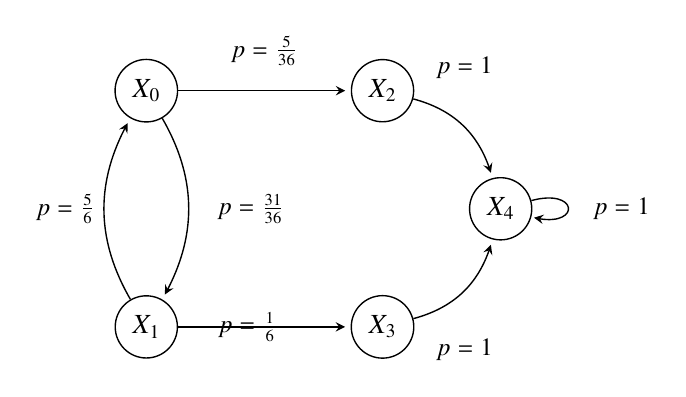
\begin{tikzpicture}[->, >= stealth, shorten >=2pt, line width=0.5pt, node distance=2cm]
  \node[circle, draw] (A) at (0, 3) {$X_0$};
  \node[circle, draw] (B) at (0, 0) {$X_1$};
  \node[circle, draw] (C) at (3, 3) {$X_2$};
  
  \node[circle, draw] (D) at (3, 0) {$X_3$};
  \node[circle, draw] (E) at (4.5, 1.5) {$X_4$};
  
  
  \begin{small}
    \path (A) edge [bend left]  node [left][right=0.25cm] {$p = \frac{31}{36}$} (B);
     \path (B) edge [bend left] node [left] {$p = \frac{5}{6}$} (A);
      \path (A) edge  node [left][above=0.2cm] {$p = \frac{5}{36}$} (C);
       \path (B) edge  node [left][below=0.3cm][right=-0.7cm] {$p = \frac{1}{6}$} (D);
        \path (C) edge [bend left] node [left][above=0.5cm] {$p = 1$} (E);
         \path (D) edge [bend right] node [left][below=0.5cm] {$p = 1$} (E);
         \path (E) edge [loop right] node [left] [right=0.2cm]{$p = 1$} (E);
   % \path (A) edge [bend left] node [below = 0.4cm] {$p = \frac{31}{36}\times\frac{5}{6}\times\frac{5}{36}$} (B);
    %\path (A) edge [bend right] node [below = 0.2cm] {$p = \frac{31}{36}\times\frac{5}{36}\times\frac{31}{36}$} (C);
    
    
  \end{small}
\end{tikzpicture}
}
    \caption{State diagram generated using LatexTikZ}
    \label{fig:Statediagramdiecoin}
\end{figure}
\\
Initial state vector\\
\begin{align}
\vec{S}_0 &= \myvec{ 1\\ 0\\0\\0\\0\\}
\end{align}
Transition matrix\\
\begin{align}
\vec{P} &= \myvec{
    0 & \frac{5}{6} & 0 & 0 & 0 \\
    \frac{31}{36} & 0 & 0 & 0 & 0 \\
    \frac{5}{36} & 0 & 0 & 0 & 0 \\
    0 & \frac{1}{6} & 0 & 0 & 0 \\
    0 & 0 & 1 & 1 & 1\\
}
\end{align}
Probablity of A winning in third throw given A starts first\\
\begin{align}
\vec{S}_1 &= \vec{P}\vec{S_0}\\
\vec{S_2} &= \vec{P}\vec{S_1}\\
\vec{S_3} &= \vec{P}\vec{S_2}\\
    &= \vec{P^3}\vec{S_0}\\
&= \myvec{
    \frac{775}{1296} & 0 & 0 & 0 & 0 \\
    \frac{4805}{7776} & 0 & 0 & 0 & 0 \\
    \frac{775}{7776} & 0 & 0 & 0 & 0 \\
    0 & \frac{155}{1296} & 0 & 0 & 0 \\
    \frac{61}{216} & \frac{61}{216} & 1 & 1 & 1
}
\myvec{ 1\\ 0\\0\\0\\0\\}\\
\vec{S_3} &= \myvec{0.597\\ 0.617\\0.099\\0\\0.282}\\
\vec{S_3}[2] &= 0.099
\end{align}


